%%%%%%%%%%%%%%%%%%%%%%%%%%%%%%%%%%%%%%%%%
% Beamer Presentation
% LaTeX Template
% Version 1.0 (10/11/12)
%
% This template has been downloaded from:
% http://www.LaTeXTemplates.com
%
% License:
% CC BY-NC-SA 3.0 (http://creativecommons.org/licenses/by-nc-sa/3.0/)
%
%%%%%%%%%%%%%%%%%%%%%%%%%%%%%%%%%%%%%%%%%

%----------------------------------------------------------------------------------------
%	PACKAGES AND THEMES
%----------------------------------------------------------------------------------------

\documentclass{beamer}

\mode<presentation> {

% The Beamer class comes with a number of default slide themes
% which change the colors and layouts of slides. Below this is a list
% of all the themes, uncomment each in turn to see what they look like.

%\usetheme{default}
%\usetheme{AnnArbor}
%\usetheme{Antibes}
%\usetheme{Bergen}
%\usetheme{Berkeley}
%\usetheme{Berlin}
%\usetheme{Boadilla}
%\usetheme{CambridgeUS}
%\usetheme{Copenhagen}
%\usetheme{Darmstadt}
%\usetheme{Dresden}
%\usetheme{Frankfurt}
%\usetheme{Goettingen}
%\usetheme{Hannover}
%\usetheme{Ilmenau}
%\usetheme{JuanLesPins}
%\usetheme{Luebeck}
\usetheme{Madrid}
%\usetheme{Malmoe}
%\usetheme{Marburg}
%\usetheme{Montpellier}
%\usetheme{PaloAlto}
%\usetheme{Pittsburgh}
%\usetheme{Rochester}
%\usetheme{Singapore}
%\usetheme{Szeged}
%\usetheme{Warsaw}

% As well as themes, the Beamer class has a number of color themes
% for any slide theme. Uncomment each of these in turn to see how it
% changes the colors of your current slide theme.

%\usecolortheme{albatross}
%\usecolortheme{beaver}
%\usecolortheme{beetle}
%\usecolortheme{crane}
%\usecolortheme{dolphin}
%\usecolortheme{dove}
%\usecolortheme{fly}
%\usecolortheme{lily}
%\usecolortheme{orchid}
%\usecolortheme{rose}
%\usecolortheme{seagull}
%\usecolortheme{seahorse}
%\usecolortheme{whale}
%\usecolortheme{wolverine}T

%\setbeamertemplate{footline} % To remove the footer line in all slides uncomment this line
%\setbeamertemplate{footline}[page number] % To replace the footer line in all slides with a simple slide count uncomment this line

%\setbeamertemplate{navigation symbols}{} % To remove the navigation symbols from the bottom of all slides uncomment this line
}

\usepackage{graphicx} % Allows including images
\usepackage{booktabs} % Allows the use of \toprule, \midrule and \bottomrule in tables
\usepackage{parskip}

\setbeamersize{text margin left=5.5mm,text margin right=5.5mm} 


%----------------------------------------------------------------------------------------
%	TITLE PAGE
%----------------------------------------------------------------------------------------

\title[Discrete Logarithm]{Discrete Logarithm: ElGamal, Algorithms, Practice} % The short title appears at the bottom of every slide, the full title is only on the title page

\author{Ilaria Battiston} % Your name
\institute[TUM] % Your institution as it will appear on the bottom of every slide, may be shorthand to save space
{
Technical University Munich \\ % Your institution for the title page
\medskip
\textit{i.battiston@tum.de} % Your email address
}
\date{June 23, 2020} % Date, can be changed to a custom date

\begin{document}

\begin{frame}
\titlepage % Print the title page as the first slide
\end{frame}

\begin{frame}
\frametitle{Overview} % Table of contents slide, comment this block out to remove it
\begin{minipage}{4in}
    \tableofcontents
  \end{minipage} % Throughout your presentation, if you choose to use \section{} and \subsection{} commands, these will automatically be printed on this slide as an overview of your presentation
\end{frame}

%----------------------------------------------------------------------------------------
%	PRESENTATION SLIDES
%----------------------------------------------------------------------------------------

%------------------------------------------------
\section{The Discrete Logarithm} % Sections can be created in order to organize your presentation into discrete blocks, all sections and subsections are automatically printed in the table of contents as an overview of the talk
%------------------------------------------------
\subsection{Functioning and examples} % A subsection can be created just before a set of slides with a common theme to further break down your presentation into chunks
\subsection{Computational aspects and real life applications}

\begin{frame}
\frametitle{The Discrete Logarithm}
The discrete logarithm is a public key cryptosystem proposed in the 1970s taking advantage of the infeasibility of inverse logarithms within finite cyclic groups.
\bigskip
\begin{block}{Discrete Logarithm}
If $G$ is a finite group, $b$ is an element of $G$, and $y$ is an element of $G$ which is a power of $b$, then the discrete logarithm of $y$ to the base $b$ is any integer $x$ such that $b^x = y$.
\end{block}

\end{frame}

%------------------------------------------------

\begin{frame}
\frametitle{Infeasibility of the discrete logarithm}
Having a finite cyclic group $\mathbb{Z}^*_p$ of order $p - 1$, taking a primitive element $\alpha \in\mathbb{Z}^*_p$ and another element $\beta \in \mathbb{Z}^*_p$, the discrete logarithm problem aims to determine the integer $1 \leq x \leq p - 1$ such that:
$$\alpha^x \equiv \beta \mod p \qquad \rightarrow \qquad x = \log_\alpha\beta \mod p$$

Raising a number $b$ to a power $x$ in a large finite field is an one-way function, i.e.\ it is far more difficult to apply the inverse operation and finding $\log_bx$. 

Given an element $y = b^x$, finding $y$ is therefore an open problem.
\end{frame}

%------------------------------------------------

\begin{frame}
\frametitle{Discrete Logarithm computation}

\begin{example}
Considering a discrete logarithm in the group $\mathbb{Z}^*_{47}$, in which $\alpha = 5$ is a primitive element, the aim is finding the positive integer $x$ such that $5^x \equiv 41 \mod 47$.
\vspace{0.3cm}
A brute-force attack reveals that the result is $x = 15$.
Using prime cardinality is important in order to avoid potential attacks.
\end{example}

\end{frame}

%------------------------------------------------

\begin{frame}
\frametitle{Computational aspects}
Influencing computation:
\begin{itemize}
    \item Finite fields in which discrete logarithm is computed
    \item Length of involved operands
    \item Repeated exponentiation
\end{itemize}
Performance can be a problem creating serious bottleneck in devices with small CPUs.
\end{frame}

%------------------------------------------------

\begin{frame}
\frametitle{Security}
\begin{table}
\begin{tabular}{l l}
\textbf{Bit lengths} & \textbf{Security level} \\
\midrule
1024 bit & 80 bit \\
3072 bit & 128 bit \\
7680 bit & 192 bit \\
15360 bit & 256 bit
\end{tabular}
\medskip
\caption{Different security levels for discrete logarithm [Paar]}
\end{table}
\end{frame}

%------------------------------------------------

\begin{frame}
\frametitle{Practical applications}
\begin{itemize}
    \item Standardized by the Internet Key Exchange
    \item LAN security
    \item Authentication and confidentiality protection
    \item Diffie-Hellman key exchange
\end{itemize}
\end{frame}

%------------------------------------------------
\section{The Diffie-Hellman key exchange}
\subsection{Protocol}
\subsection{Security}
%------------------------------------------------

\begin{frame}
\frametitle{Quiz}
Which one of these is NOT an advantage of public key cryptography?
\bigskip
\begin{description}
    \item[A.] Secure information through insecure channel
    \item[B.] Computational speed of encryption and decryption
    \item[C.] Robust authentication
\end{description}

\end{frame}

%------------------------------------------------

\begin{frame}
\frametitle{The Diffie-Hellman key exchange}
Diffie-Hellman is a schema used to exchange private keys through public key cryptography, based on \textbf{commutativity of exponentiation} within prime fields.

\begin{itemize}
    \item Computationally faster operations since public key encryption is only performed once
    \item Secure identity establishment
    \item Third parties cannot retrieve original values
    \item Can be used by more than two parts
\end{itemize}


\end{frame}

%------------------------------------------------

\begin{frame}
\frametitle{How it works}
\begin{figure}
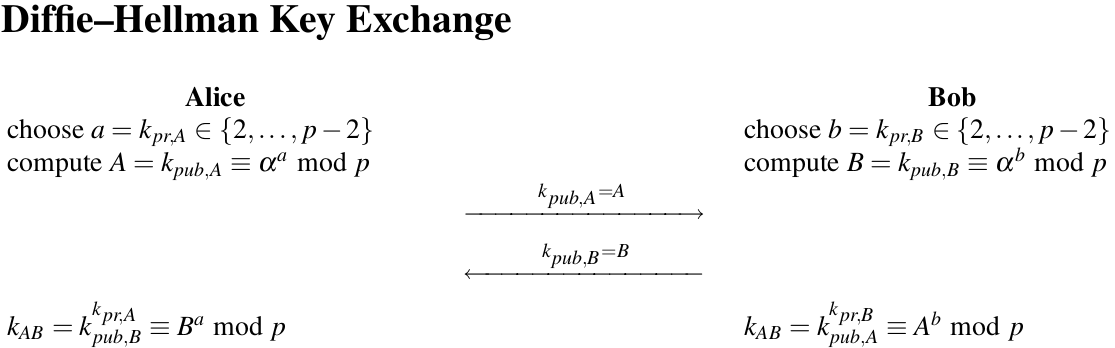
\includegraphics[width=1\linewidth]{DiffieHellmanPaarCropped.png}
\caption{Key exchange between Alice and Bob [Paar]}
\end{figure}
\[ (\alpha^a)^b = (\alpha^b)^a \]
\end{frame}

%------------------------------------------------

\begin{frame}
\frametitle{Attacks}

\begin{columns}[c] % The "c" option specifies centered vertical alignment while the "t" option is used for top vertical alignment

\column{.45\textwidth} % Left column and width
\textbf{Passive attacks}
\begin{itemize}
\item Man-in-the-middle
\end{itemize}

\column{.5\textwidth} % Right column and width
\textbf{Active attacks}
\begin{itemize}
\item Discrete Log Computation
\end{itemize}
\end{columns}
\medskip
The discrete logarithm computation is the only available method to crack Diffie-Hellman, however this is infeasible among groups with large prime factors dividing their cardinality.

\end{frame}

%------------------------------------------------

\begin{frame}
\frametitle{Applications}
DHKE, thanks to its many advantages, is widely used in practice:
\begin{itemize}
    \item SSH, providing security between client-server architectures
    \item TLS, encrypting communication between computer networks
    \item IpSec, establishing authentication among virtual private networks
\end{itemize}

\end{frame}

%------------------------------------------------

\begin{frame}
\frametitle{Vulnerabilities}
\begin{columns}[c]
\column{.45\textwidth} % Left column and width
\textbf{Commonly used groups}
Internet traffic mostly relies on commonly-known groups, involving primes with less than 1024 bits, to reduce computational complexity and increase interoperability.

\column{.5\textwidth} % Right column and width
\textbf{Logjam attack}\\
Logjam exploits usage of these groups to compute 512-bit keys discrete logarithms among commonly-used groups. After the initial phase of precomputation, keys could be cracked within minutes.
\end{columns}

\end{frame}



%------------------------------------------------
\section{The ElGamal Cryotosystem}
\subsection{Protocol and proof}
\subsection{Computation and security}
%------------------------------------------------

\begin{frame}
\frametitle{The ElGamal Cryptosystem}
The ElGamal cryptosystem is an encryption scheme that can also be applied in general cyclic groups.

Its key aspect is the \textbf{randomized encryption}: Diffie-Hellman requires interaction of both parties to calculate a common private key. 

This can constitute in a problem in case they are not able to interact, due to delays in transmission or unavailability of receiver.

The random exponent is therefore introduced to replace the private exponent of the receiving entity, so that it does not have to take part in the exchange.

\end{frame}

%------------------------------------------------

\begin{frame}
\frametitle{The ElGamal Protocol}

\begin{figure}
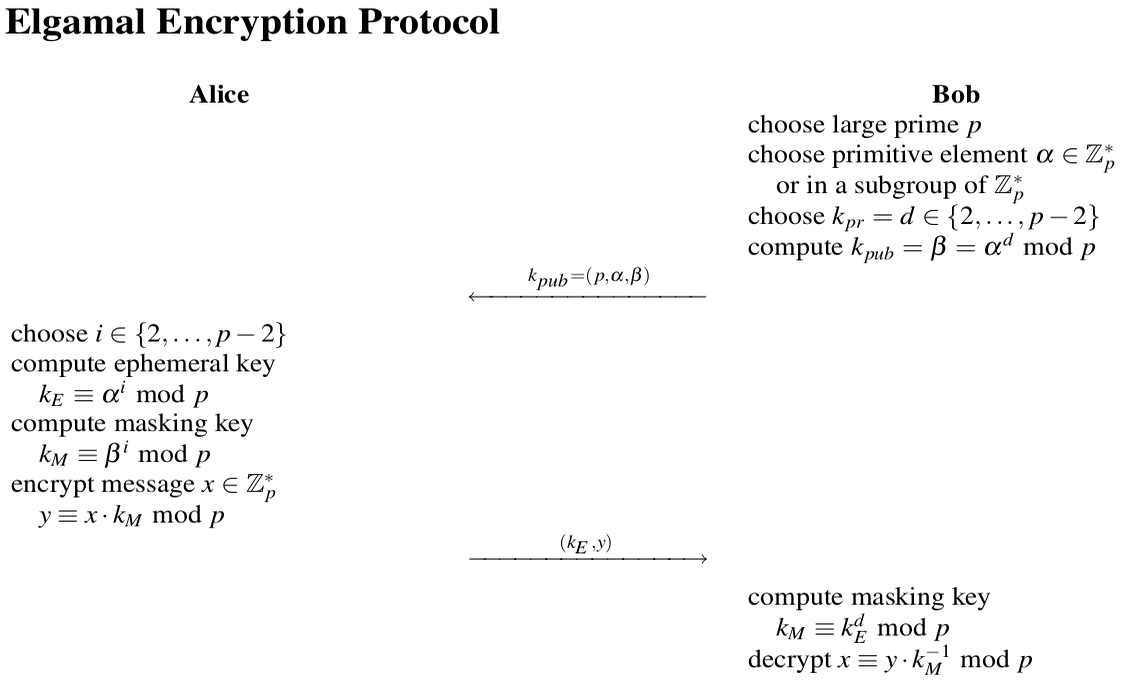
\includegraphics[width=0.95\linewidth]{ElGamalPaarCropped.png}
\caption{ElGamal key exchange between Alice and Bob [Paar]}
\end{figure}

\end{frame}

%------------------------------------------------

\begin{frame}
\frametitle{Proof}
\[y = x \cdot \alpha^{id} \qquad k_M = \alpha^{di} \qquad k_E = \alpha^i \]

\begin{equation}
\begin{split}
d_{k_{pr}}(k_E, y) &\equiv y \cdot (k_M)^{-1} \mod p \\
&\equiv [x \cdot k_M] \cdot (k_E^d)^{-1} \mod p \\
&\equiv (x \cdot \alpha^{id}) \cdot (\alpha^{id})^{-1} \mod p \\
&\equiv [x \cdot (\alpha^d)^i]^{-1} \mod p \\
&\equiv x \cdot \alpha^{d \cdot i - d \cdot i} \mod p \\
&\equiv x \mod p
\end{split}
\end{equation}

\end{frame}

%------------------------------------------------

\begin{frame}
\frametitle{Computation}

The ciphertext is twice as long as the message: therefore, the message expansion factor of ElGamal is two. 

ElGamal  is a \textbf{probabilistic encryption scheme}: encrypting two identical messages $x_1, x_2$ using the same public key results with \textit{extremely high likelihood} in two different ciphertexts $y_1 \neq y_2$. 

The random exponent $i$, however, \textbf{should not be reused}: the two masking keys would be the same, along with the ephemeral keys.

Two identical cyphertexts $(y_1, k_E)$ are therefore sent through the channel. If an attacker can guess the first message, the second one can be computed as well using the same masking key.

\end{frame}

%------------------------------------------------

\begin{frame}
\frametitle{Practical issues}
ElGamal encryption is not widely used in practice, since one of the best known practices to break it exploits its malleability: the ciphertext $(k_E, y)$ can be replaced with $(k_E, sy)$ for some integer $s$.

The receiver therefore then computes:
\begin{equation}
\begin{split}
d_{k_{pr}}(k_E, sy) &\equiv sy \cdot (k_M)^{-1} \mod p \\
&\equiv s \cdot (x \cdot k_M) \cdot k_M^{-1} \mod p \\
&\equiv sx \mod p
\end{split}
\end{equation}

The decrypted text is also a multiple of $s$, and although an attacker would not be able to decrypt the message, he is able to manipulate it and compromise communication.

\end{frame}

%------------------------------------------------

\begin{frame}
\frametitle{Applications and security}

The ElGamal encryption system is used in GNU Privacy Guard System and recent versions of PGP, however the exponent has to be large enough or those systems will be subject to vulnerabilities.

Despite being easy to manipulate, the cryptography is secure. The only  active ways an attacker can break the ElGamal scheme are:
\begin{enumerate}
	\item Finding $d$, i.e.\ computing $d = \log_\alpha \beta \mod p$, which is computationally infeasible
	\item Trying to guess the random exponent $i = log_\alpha k \mod p$, which still involves solving the discrete logarithm problem
\end{enumerate}
  
\end{frame}

%------------------------------------------------

\begin{frame}
\frametitle{Quiz}
Which of these characteristics correspond to Diffie-Hellman, which ones to ElGamal and which ones to both?
\begin{enumerate}
    \item Used in TLS
    \item Based on discrete logarithm
    \item Randomized exponentiation
    \item Mainly used for key exchange
    \item Probabilistic algorithm
    \item Can be used by more than two parts
\end{enumerate}
\end{frame}

%------------------------------------------------

\section{Algorithms to find Discrete Logarithm}
\subsection{Pollard Rho}
\subsection{Index Calculus}

\begin{frame}
\frametitle{Theoretical bounds}
Attacks against discrete logarithm involve finding the integer $x$ for a given $\alpha$ and $\beta$ in $G$ such that:
$$\beta = \alpha \circ \alpha \circ \dots \circ \ alpha = \alpha^x$$

A generic algorithm that solves \textit{with high probability} the problem must perform at least $\Omega(p^{1/2})$ group operations, where $p$ is the largest prime dividing the cardinality of the group. 

In 2019 by a group of researchers who announced the computation of the discrete logarithm of a number composed by 795 bit. This was obtained using a 2.1GHz CPU and took approximately 4000 core-years.

\end{frame}

%------------------------------------------------

\begin{frame}
\frametitle{Pollard Rho}
Based on the \textbf{birthday paradox}: the basic idea consists in pseudo-randomly generate group elements of the form $\alpha^i \cdot \beta^j$, keeping track of values $i$ and $j$, to then continue until obtaining a collision:
$$\alpha^{i_1} \cdot \beta^{j_1} = \alpha^{i_2} \cdot \beta^{j_2}$$
Substituting $\beta = \alpha^x$ and comparing the exponents on both sides of the equation, the collision leads to the following formula:
$$i_1 + xj_1 \equiv i_2 + jx_2 \mod |G| \qquad \rightarrow \qquad x \equiv \frac{i_2 - i_1}{j_1 - j_2} \mod |G|$$ 
\end{frame}

%------------------------------------------------

\begin{frame}
\frametitle{Index-calculus}

Probablistic algorithm taking advantage of high parallelism, one of the most efficient methods to find discrete logarithms within polynomial groups.

Here, the term \textbf{index} is a commonly used word to define the discrete logarithm: $x = ind(a) \mod q$ for some base $b$, for $b^x \equiv a \mod m$.

Index-calculus depends on the property that a significant fraction of elements of $G$ can be efficiently expressed as \textbf{products of elements} of a small subset of $G$, assuming $|G|= q = p^n$ is a fairly large power of a small prime $p$. 

\end{frame}

%------------------------------------------------

\begin{frame}
\frametitle{Index-calculus: precomputation}

An irreducible element $f \in \mathbb{Z}^*_q$ is identified, and a subset $B \subset \mathbb{Z}^*_q$ is chosen.

Then, a random integer $t \in [1, q - 2]$ is chosen and then $b^t \in \mathbb{Z}^*_q$ is computed through repeated squaring. The algorithm finds all elements $c \in \mathbb{Z}^*_q$ such that:
$$c = b^t \mod f$$

Now, the index-calculus algorithm attempts to write $c$ as:
$$c = c_0 \prod_{a \in B} a ^{m}$$
$m$ is the highest power of $a$ which divides $c$.

\end{frame}

%------------------------------------------------

\begin{frame}
\frametitle{Index-calculus: precomputation}

Now, supposing some $c \equiv b^t \mod f$ has been found, and $c$ has the desired type of factorization, taking the discrete logarithm of both sides allows to obtain:
$$ind(c) - ind(c_0) \equiv \sum_{a \in B} m \cdot ind(a) \mod q - 1$$

Repeating the process, eventually a large number of independent congruences will be found, written as:
$$t - ind(c_0) \equiv \sum_{a \in B} m \cdot ind(a) \mod q - 1$$

\end{frame}

%------------------------------------------------

\begin{frame}
\frametitle{Index-calculus: computation}

A random integer $t$ is once again chosen, and $y = xb^t$ is computed, i.e.\ the unique element $y \in \mathbb{Z}^*_q$ satisfying $y \equiv xb^t \mod f$.

As in the first stage, $y$ has to be factored until an integer is obtained such that:
$$y = y_0 \prod_{a \in B} a ^{m}$$

As soon as this happens, the algorithm can terminate:
\[ind(x) = ind(y) - t \qquad \land \qquad ind(y) = ind(y_0) + \sum_{a \in B} m \cdot ind(a)\]

This algorithm allows to obtain a runtime which is not exponential in the bit length of the order, but \textbf{subexponential}.

\end{frame}

%------------------------------------------------

\begin{frame}{Considerations}

Despite the existence of efficient algorithms running on advanced hardware, the discrete logarithm is still considered among the NP-hard problems. 

Index-calculus allows to compute discrete logarithms within groups with security level smaller than 80 bits.

1024-bit keys, however, are considered secure and unbreakable by current resources, although computational times of algorithms can be shortened by improving preprocessing and applying other mathematical properties to operations.
    
\end{frame}

%------------------------------------------------
\section{Comparison with integer factorization}
\begin{frame}
\frametitle{Comparison with integer factorization}

\begin{enumerate}
	\item Both concern cases of the small subgroup problem for finite commutative groups
	\item Both are NP-hard problems, despite the existence of efficient algorithms on quantum computers
	\item Both have been extensively used to construct strong encryption systems still valid today
	\item Algorithms are similar due to modular arithmetic
\end{enumerate}
\end{frame}

%------------------------------------------------

\begin{frame} % Need to use the fragile option when verbatim is used in the slide
\frametitle{Conclusion and open questions}

\begin{itemize}
	\item Are there better algorithms yet to be discovered?
	\item Is quantum computing an efficient way to reduce computational time?
	\item Would attacks on elliptic curves also influence discrete logarithm?
\end{itemize}
\bigskip
Having these open questions allow space for further research and development, while still ensuring computation infeasibility. 
\end{frame}

%------------------------------------------------

%------------------------------------------------

\begin{frame}
\Huge{\centerline{Thank you for your attention!}}
\end{frame}

%----------------------------------------------------------------------------------------


\begin{frame}
\frametitle{References}
\footnotesize{
\begin{thebibliography}{99} % Beamer does not support BibTeX so references must be inserted manually as below

    \bibitem{koblitz}
	N. Koblitz - A Course in Number Theory and Cryptography
	\bibitem{knuth}
	D. Knuth - The Art of Computer Programming, Vol. II
	\bibitem{paar}
	C. Paar, J. Pelzl - Understanding Cryptography
	\bibitem{shor}
	P. W. Shor - Polynomial-Time Algorithms for Prime Factorization and Discrete Logarithms on a Quantum Computer
	\bibitem{european}
	P. Horster, H Knoblock - Discrete Logarithm Based Protocols
	\bibitem{shoup}
	V. Shoup - Lower Bounds for Discrete Logarithms and Related Problems
	\bibitem{768}
	T. Kleinjung, C. Diem, A. Lenstra, C. Priplata, C. Stahlke - Computation of a 768-bit prime field discrete logarithm
	\bibitem{tls}
	D. Adrian et al. - Imperfect Forward Secrecy: How Diffie-Hellman Fails in Practice
	\bibitem{tum}
	A. Meier - The ElGamal Cryptosystem

\end{thebibliography}
}
\end{frame}

\end{document} 